\documentclass[11pt, titlepage, fleqn]{report}
\usepackage[utf8]{inputenc}
\usepackage[T1]{fontenc}
\usepackage{graphicx}
\usepackage{hyperref}
\usepackage{listings}
\usepackage{siunitx}
\usepackage[left=3cm, right=2cm, top=3cm, bottom=2cm]{geometry}
\usepackage{hsellogo}
\usepackage{hselfonts}
\usepackage{hselcolor}
\usepackage{hselmath}
\usepackage{amsmath}
\usepackage{siunitx}
\usepackage{parskip}
\usepackage{csquotes}
\usepackage{acronym}
\usepackage{wrapfig}
\usepackage{subcaption}
\usepackage{float}
\usepackage{hyphenat}
\usepackage[ngerman, german]{babel}
\usepackage[citestyle=numeric,bibstyle=numeric, sorting = none,
hyperref=true,backref=true,maxcitenames=3,url=true,backend=biber,natbib=true]{biblatex}
\addbibresource{references.bib}
\author{Liebenow, Wozasek}
\date{\textit{<2020-01-26 Sun>}}
\title{Dokumentation HoloOSCv2\\\medskip
\large Dokumentation HoloOSCv2}
\DeclareMathOperator{\atantwo}{atan2}
 
\begin{document}


    \begin{titlepage}% Deckblattk
        \hsellogo\hfill Projektgruppe % etwa Bachelorarbeit, Masterarbeit
        \par
        \vspace{4cm}
        \noindent\parbox{0.8\textwidth}{\Huge HoloOSCv2 - Dokumentation}  
        \vspace{2cm}

        \Large \noindent vorgelegt von:
        \begin{itemize}
            \item Tino Liebenow - Matrikelnummer 7011830
            \item Justin Wozasek - Matrikelnummer 7011366
            \item Nils Münke - Matrikelnummer 7010176
            \item Jan  Samus - Matrikelnummer 7009617
            \item Jannik Indorf - Matrikelnummer 7010475
        \end{itemize}
        \vspace{2cm}
        betreut duch\newline
        Prof. Dr.-Ing. Johann-Markus Batke\newline
        Abgabedatum: 30.01.2020
    \end{titlepage}
    \newpage
    \tableofcontents % Inhaltsverzeichnis
    \listoffigures% Abbildungsverzeichnis
    \newpage
    \section*{\Huge Abkürzungsverzeichnis}% Abkürzungen
    \label{sec:Abkürzungsverzeichnis}
    \vspace{1cm}
    \begin{acronym}
        \acro{ar}[AR]{Augmented Reality}
        \acro{daw}[DAW]{Digital Audio Workstation}
        \acro{hsel}[HSEL]{Hochschule Emden Leer}
        \acro{htc}[HTC]{High Tech Computer - taiwanischer Computerhersteller}
        \acro{iem}[IEM]{Institute of Electronic Music and Acoustics}
        \acro{mr}[MR]{Mixed Reality}
        \acro{mrtk}[MRTK]{Mixed Reality Toolkit}
        \acro{osc}[OSC]{Open Sound Control}
        \acro{vr}[VR]{Virtual Reality}
    \end{acronym}  
    \newpage
    \chapter{Einleitung}% Kapitel 1
    \label{sec:Einleitung} 
     	\sloppy \nohyphens{
        Die fortschreitende Entwicklung von virtuellen 3-D technischen Systemen hat in den letzten Jahren in vielen Bereichen große Sprünge ermöglicht. So unterstütze ein 
        derartiges System zuletzt die erfolgreiche Durchführung einer Herzoperation in Polen und assistierte den Chirurgen mittels einer dreidimensionalen computertomografischen 
        Projektion. Dieses Beispiel zeigt das Potenzial besagter Systeme, den Bereich der visuellen Wahrnehmung massiv zu erweitern. 
        \newline Ähnliches gilt in der 3D-Audio-Bearbeitung. 
        So sind die meisten Anwendungen noch auf zweidimensionale Bildschirme begrenzt, wodurch die akustische und visuelle Wahrnehmung nur selektiv beansprucht wird. 
        In diesem Projekt wird daher die Digital Audio Workstation (DAW) Reaper 
        unter Verwendung der Microsoft HoloLens und eines 360° 
        Lautsprechersystems durch ein virtuelles 
        dreidimensionales Interface erweitert um eine räumliche 
        Audiobearbeitung zu ermöglichen und somit die auditive und visuelle 
        Wahrnehmung zu synergieren.\newline
        Im Folgenden wird zunächst die zugrunde liegende Theorie erklärt und die verwendete Hard- und Software vorgestellt. Anschließend werden die einzelnen resultierenden 
        Aufgabengebiete definiert und schlussendlich die erreichten Ziele 
        beschrieben.\vspace{\baselineskip}\newline
        Aus Gründen der Lesbarkeit wurde in dieser Arbeit die männliche Form 
        für Personenbeschreibungen genutzt. Diese beziehen sich trotzdem auf 
        Angehörige aller Geschlechter/Gender. \newline
        Da in dieser Arbeit keine Buchquellen vorkommen und viele Quellen keine 
        Autoren aufweisen, sind die Verweise in der Form "'[<Erläuterung der 
        Quelle> [<Verweisnummer>]]"' dargestellt.\newline
    	}
    \chapter{Theorie}% Kapitel 2
    \label{sec:Theorie}
    	Im folgenden Kapitel werden die theoretischen Grundlagen zu dieser 
    	Arbeit betrachtet. Dabei wird auf Augmented Reality, 3-D-Audio und die 
    	verwendete Hard- und Software eingegangen.
        \section{Augmented Reality}
        \label{sec:2.1}
            Unter erweiterter Realität (Augmented Reality, AR) versteht man die 
            Kombination aus wahrgenommener und vom Computer erzeugter Realität.
            Oft wird in den öffentlichen Medien für die erweiterte Realität der Begriff “Mixed Reality” (MR) verwendet, obwohl Mixed Reality von der erweiterten 
            Realität abzugrenzen ist. Zur Mixed Reality gehören auch andere Technologien wie die weitgehend unbekannte erweiterte Virtualität (Augmented Virtuality, 
            AV) und die virtuelle Realität (Virtual Reality, VR).
            \begin{figure}[htbp]
                \centering
                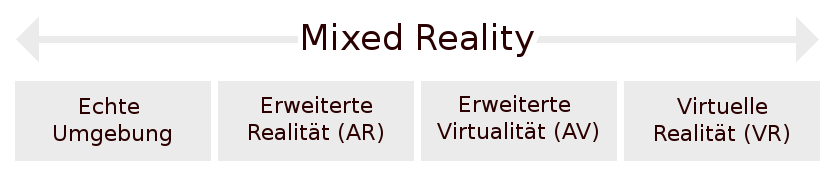
\includegraphics[width=\linewidth]{./img/Mixed_Reality.png}
                \caption[Bestandteile der Mixed Reality]{Bestandteile der Mixed Reality [Tinkla \cite{MR}] \label{fig:MRPic}}
            \end{figure}
            \newline Im Gegensatz zur virtuellen Realität geht es bei der erweiterten Realität darum, dem Nutzer zusätzlich zur wahrgenommenen Realität ergänzende 
            Zusatzinformationen zur Verfügung zu stellen.
            Angefangen wurde mit ersten AR-Anwendungen im Sport: Live-Videos wurden durch Computergrafiken und -animationen erweitert. 
            Bewegte Linien wurden bei bestimmten Bewegungsabläufen eingeblendet. So können beispielsweise Laufwege von Fußballspielern verdeutlicht werden.
            \newline Neuere Entwicklungen befassen sich mit der Mobilkommunikation und unterstützen die Benutzer durch Zusatzinformationen beispielsweise bei der Navigation.
            Für dieses Beispiel sind die Programme darauf ausgelegt, dass der 
            Benutzer die Kamera des Smartphones auf den Straßenverkehr richtet. 
            Dem Benutzer wird 
            dann auf dem Display des mobilen Geräts ein Navigationssystem angezeigt. Die Darstellung wird durch Bilderkennung und Ortung des mobilen Geräts ermöglicht.
            Andere Anwendungsmöglichkeiten, als mit einem mobilen Gerät, finden sich bei der Verwendung eines Head-mounted-Displays, wie beispielsweise die Microsoft 
            HoloLens.\newline
            Head-mounted-Displays werden umgangssprachlich auch AR-Brillen genannt, da sie dem Nutzer auf den Kopf gesetzt werden und dieser dann durch ein Display 
            schaut. Je nach Programm werden dem Nutzer daraufhin 
            Zusatzinformationen über das Display eingeblendet. Diese Technik 
            findet in Flugsimulatoren oder in der 
            Automotive-Technik statt, beispielsweise zur Schulung von 
            Mitarbeitern.  [Augmented Reality \cite{AR}]
        \section{3D-Audio}
            Aktuelle Surround-Systeme bieten eine gute Klangerfahrung, 
            allerdings fehlen diesen einige Elemente, um eine Erfahrung wie bei 
            einem Live-Konzert zu bieten.  [AudioLabs \cite{AudioLabs}]\newline
            3D-Audio stellt eine Wiedergabetechnik dar, die realistischer wirkende Audio-Erfahrungen bieten kann als konventionelle 5.1 oder 7.1 Surround-Systeme.
            Die Lautsprecher sind im Gegensatz zu konventionellen Systemen in 
            drei verschiedenen Ebenen der Höhe angeordnet und umschließen den 
            Nutzer, der sich im optimalen Fall genau mittig des Systems 
            befindet.
            In diesem Projekt werden Audioquellen der Szene hinzugefügt und können um den Nutzer, der sich innerhalb des 3D-Audiosystems befindet, frei bewegt werden. In Verbindung mit der Microsoft 
            HoloLens wird dem Nutzer somit eine Erfahrung geboten, die Audioquelle zu sehen und das sichtbare Audio-Objekt frei um sich herum zu positionieren.       
        \label{sec:2.2}
   
        \section{Verwendete Hard- und Software}
        \label{sec:2.3}
        	\begin{figure}[H]
        		\centering
        		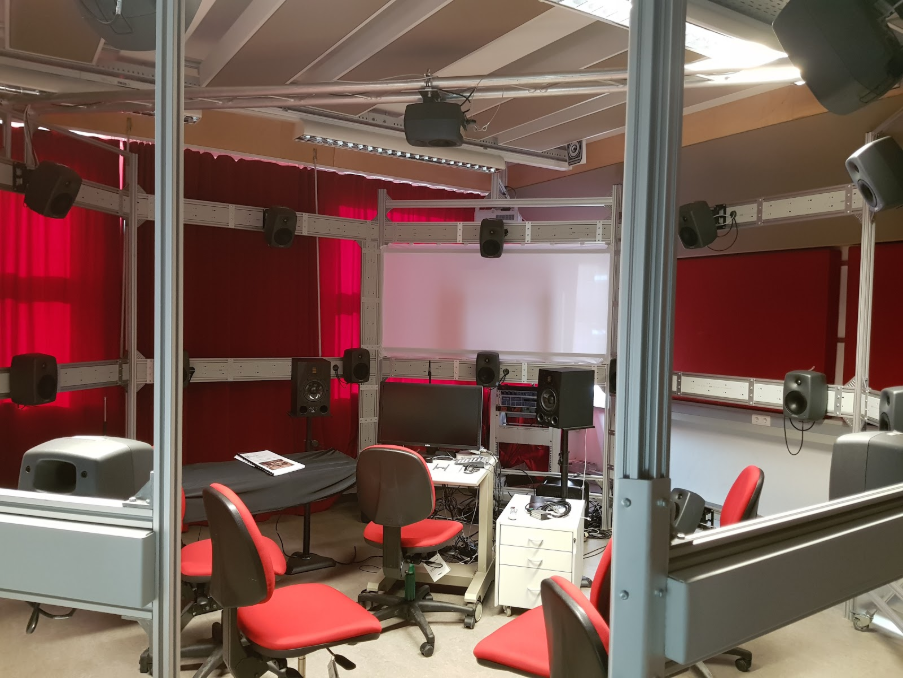
\includegraphics[height=8.5cm]{./img/Studio.png}
        		\caption[3D-Audio-Labor an der HSEL]{3D-Audio-Labor an der HSEL (Stand: 
        		01/2020)\label{fig:MR}}
        	\end{figure}
            \subsection{Audio}
            \label{sec:2.3.1 Audio}
                \subsubsection{Lautsprechersystem an der HSEL}
                    Um 3D-Audio wiedergeben zu können, wird eine spezielle Lautsprecheranordnung benötigt. Die Hochschule Emden/Leer (HSEL) besitzt ein 
                    22.2 Lautsprechersystem (Abb. \ref{fig:MR}), dass für 
                    dieses Projekt 
                    genutzt worden ist. Es entstand im Rahmen einer 
                    studentischen Projektarbeit und entspricht 
                    der Norm ITU-R BS.2159-7 von der International Telecommunication Union für ein 22.2 Lautsprecher-System.
                    Bedient wird das System von einem Computer inmitten des Lautsprecher-Systems, welcher über Reaper die einzelnen Lautsprecher ansprechen kann.
                    
                \subsubsection{Reaper}
                \label{sec:Reaper}
                    Reaper ist eine digitale Audio-Produktions-Applikation, 
                    welche unter Anderem für Midi-Aufnahmen, Editierung, 
                    Verarbeitung, Mixing und Mastering 
                    genutzt wird. [Reaper \cite{Reaper}]\newline 
                    Reaper kann durch die Unterstützung vieler Plugins und Hardware erweitert werden und wird im Audiolabor zur Ansteuerung des Lautsprechersystems genutzt.
                    Im Projekt wird Reaper Version 5.985 genutzt, zur Zeit der 
                    Anfertigung dieser Dokumentation ist Reaper 6.03 bereits 
                    verfügbar. Anders als bei anderen 
                    Softwarekomponenten in diesem Projekt ist die Version, in der Reaper genutzt wird, nicht ausschlaggebend.                
                \subsubsection{IEM Plug-in Suite}
                \label{sec:Suite}
                    Die IEM Plug-in Suite ist eine Open-Source Audio-Plug-in 
                    Sammlung, mit Ambisonic Plug-ins bis zur 7. Ordnung. 
                    Erstellt und gewartet wird sie vom Institute of 
                    Electronic Music and Acoustics. [IEM \cite{IEM}]\newline
                    Das Projekt nutzt die IEM Plug-in Suite 1.11.0 vom 
                    15.November 2019. Diese Version ist essenziell für das 
                    Projekt, da in ihr jedes 
                    Plug-in die Möglichkeit erhalten hat, via OSC Informationen 
                    zu senden. Zur Nutzung der erstellten Applikation ist es 
                    daher notwendig, mindestens 
                    die IEM Plug-in Suite 1.11.0 zu installieren.                
                \subsubsection{IEM-MultiEncoder}
                \label{sec:secMultiEncoder}
                    Mit dem MultiEncoder können mehrere Quellen in einem Plugin encodiert werden. Dazu kann der Nutzer oben links im Plugin die gewünschte 
                    Anzahl der Quellen wählen und diese dann nach eigenen Wünschen unter den Encoder settings im jeweiligen Azimuth, Elevation und Gain ändern. 
                    Ebenso hat der Nutzer die Möglichkeit, jede Quelle zu muten, solo auszuwählen, oder auch die ganze Kugelhülle zu bewegen.
                    Ebenso ist es möglich, wie mit allen Plugins der IEM 
                    Plug-in Suite, OSC-Nachrichten zu senden und zu empfangen.
                    \vspace{.25cm}
                    \begin{figure}[htbp]
                        \centering
                        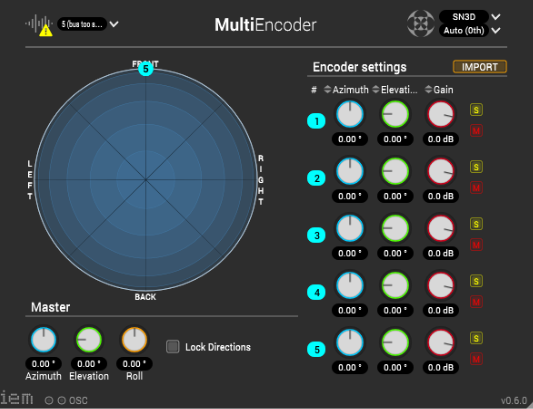
\includegraphics[height=5.5cm]{./img/MultiEncoder.png}
                        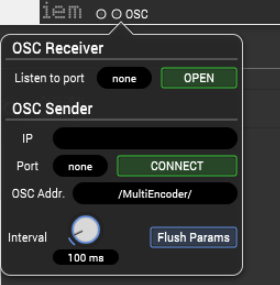
\includegraphics[height=5.5cm]{./img/MultiEncoderOSC.png}
                        \caption{Bedienoberfläche des IEM MultiEncoders \label{fig:MultiEncoder}}
                    \end{figure}
                    \subsection{Video}
            \label{sec:2.3.2Video}
                \subsubsection{HoloLens}
                    Die Microsoft HoloLens ist eine Mixed-Reality Brille, durch die der Nutzer interaktive 3D-Projektionen in der Umgebung darstellen kann.
                    [Wikipedia: HoloLens \cite{HoloLens}]\newline
                    Die HoloLens kommt - anders als viele Mitbewerber - ohne zusätzlichen Computer oder Smartphone aus.
                    Als Betriebssystem dient das Microsoft-eigene Windows 10, allerdings eine auf Mixed-Reality-Anwendungen zugeschnittene Version.
                    Die HoloLens verfügt über mehrere Sensoren, eine Kamera und zwei Lautsprecher.
                    Über die Sensoren und die Kamera kann die Brille Handgesten 
                    des Nutzers deuten und die räumlichen Gegebenheiten 
                    analysieren.
                    2019 stellte Microsoft die weiterentwickelte HoloLens 2 vor. Diese wird seit November 2019 ausgeliefert, leidet aber zur Zeit 
                    (stand: Januar 2020) noch immer unter Lieferschwierigkeiten 
                    durch eine hohe Nachfrage [Mixed \cite{Mixed}]. Die 
                    HoloLens 2 zeichnet sich durch 
                    ein größeres Display, Erkennung von Fingern und einem höheren Tragekomfort aus.
                    Zur Bedienung der HoloLens sind Gesten notwendig (Abb. 
                    \ref{fig:Gestures}).
                    \begin{figure*}[htbp]
                        \begin{subfigure}{0.5\textwidth}
                        	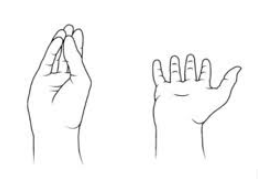
\includegraphics[height=4cm]{./img/Gesture1.png}
                        	\caption{Geste "'Blume"' zum Öffnen des Menüs}
                        \end{subfigure}
                    	\begin{subfigure}{0.5\textwidth}
                        	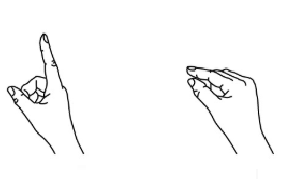
\includegraphics[height=4cm]{./img/Gesture2.png}
                        	\caption{Geste "'Tap"' zum Bestätigen oder Greifen}
                        \end{subfigure}
                        \caption[Gesten zur Bedienung der HoloLens]{Gesten zur Bedienung der HoloLens [Microsoft \cite{Gesture}]
                        \label{fig:Gestures}}
                    \end{figure*}
                \subsubsection{Mixed Reality Toolkit}
                    Das Mixed Reality Toolkit ist eine von Microsoft erstellte Sammlung von Software-Komponenten, um möglichst schnell und einfach 
                    Mixed-Reality (AR und VR) Applikationen zu erstellen. [MRTK 
                    \cite{MRTK}]\newline
                    Das MRTK ist nutzbar zur Entwicklung für die Microsoft 
                    HoloLens, die Microsoft HoloLens 2, Windows Mixed Reality 
                    Headsets und OpenVR 
                    Headsets wie die HTC Vive oder Oculus Rift.
                    Für dieses Projekt wird Version 2.0.0 genutzt. Ältere 
                    Versionen sind mit diesem Projekt wahrscheinlich nicht 
                    kompatibel, 
                    auch neuere Versionen (aktuell neuste Version: 2.1.0) können Änderungen enthalten, die nicht abwärtskompatibel sind und 
                    somit eine Umstrukturierung des Projekts nötig ist.\newline
                    Das MRTK hilft den Entwicklern bei der Erstellung von Komponenten, die in jeder Mixed Reality Applikation benötigt werden, 
                    wie beispielsweise Schaltflächen oder Verhaltensweisen von 
                    Objekten bei deren Berührung. Dazu werden die zur Verfügung 
                    stehenden Skripte
                     seitens Microsoft einfach den gewünschten Objekten in der Szene hinzugefügt und nach den Bedürfnissen des Entwicklers angepasst.
                
                \subsubsection{Unity}
                    Unity ist eine Laufzeit- und Entwicklungsumgebung für Spiele des Unternehmens Unity Technologies. Mit Unity können 2D- und 
                    3D-Applikationen für Windows, Linux, Mac und gängige 
                    Spielekonsolen erstellt werden [Wikipedia: Unity 
                    (Spiel-Engine) \cite{Unity-Engine}] und ist neben der 
                    Unreal Engine, Frostbite und CryEngine eine der am 
                    häufigsten verwendeten Spiele-Engines. [Wikipedia: 
                    Spiel-Engine 
                    \cite{Spiel-Engine}]\newline
                    Allerdings ist Unity nicht nur für Spiele geeignet, sondern 
                    kann ebenfalls für Film und Animation, oder auch für Mixed 
                    Reality Anwendungen genutzt werden. [Unity \cite{Unity}] 
                    \newline
                    Die Entwicklungsumgebung Unity ist ähnlich einer 
                    herkömmlichen Animationssoftware aufgebaut. Das 
                    Hauptfenster stellt eine Szene dar,
                    der sogenannte “GameObjects” hinzugefügt werden können. Den 
                    GameObjects können Komponenten (Materialien, Klänge, 
                    physikalische Eigenschaften, 
                    Code-Skripte) hinzugefügt werden, durch die die Szene 
                    individuell gestaltet werden kann.\newline
                    Das Projekt verwendet Unity in der Version 2019.2.2f1. 
                    Diese Version ist essenziell zur Verwendung des Projekts. 
                    Unity hat einen 
                    Aktualisierungszyklus von ungefähr zwei Wochen für eine neue Version, allerdings ist es gegebenenfalls nötig alle Assets neu 
                    zu importieren, sofern der Entwickler die Unity-Version aktualisiert.
            \subsection{Datenübertragung}
            \label{sec:2.3.3Daten}
                Open Sound Control ist ein Kommunikationsprotokoll zwischen Computern, Synthesizern und anderen Multimedia-Geräten zur Kommunikation 
                zwischen den Geräten über ein Netzwerk. [OSC \cite{OSC}]\newline
                OSC ist der Standard zur Übertragung von Audio-basierten Daten und wird von den gängigen DAWs unterstützt. 
                Dieses Projekt verwendet OSC zur Übertragung von Daten zwischen der DAW Reaper und der HoloLens. Um OSC in Unity zu verwenden, 
                wird die Software OSC simpl (for Unity) verwendet.
                \subsubsection{OSC Simpl}
                OSC simpl ist ein Unity Asset Store Produkt der dänischen 
                Designsberatung Sixth Sensor [Sixth Sensor 
                \cite{sixth-sensor}]. 
                Zur Implementierung von OSC schlägt die Seite 
                opensoundcontrol.org das Tool OSC simpl vor, welches im Unity 
                Asset Store käuflich zu erwerben ist. [OSC simpl 
                \cite{OscSimple}]
                OSC simpl macht es dem Entwickler leicht, OSC Nachrichten zu senden und zu empfangen. Dazu erhält ein leeres GameObject zwei Skripte 
                von OSC simpl, eins zum empfangen und eins zum senden. Im Unity-Inspector müssen nur noch die Ip-Adresse und der Port des 
                Empfängers eingegeben werden, dann können Daten ausgetauscht werden. 
                    
            \subsection{Versionskontrolle}
            \label{sec:2.3.4Kontrolle}
                \subsubsection{Git}
                    Git ist ein freies, verteiltes Versionsverwaltungssystem, 
                    entwickelt unter Anderem vom Linux Gründer Linus Torvalds. 
                    [Wikipedia: Git \cite{Git}]
                    In der Softwareentwicklung ist die Versionsverwaltung in 
                    Projekten mit mehreren Entwicklern essenziell um Konflikte 
                    bei Änderungen 
                    von Textdateien, wie etwa Quelltexten, zu vermeiden und wird aus selbigen Gründen in diesem Projekt genutzt.
                    Git unterscheidet sich von anderen Versionsverwaltungssystemen unter Anderem durch eine Nicht-lineare Entwicklung, dem Fehlen eines 
                    zentralen Servers, kryptographischer Sicherheit der Projektgeschichte und vielen weiteren Funktionen.
                \subsubsection{Github}
                    Github ist ein Onlinedienst zur Bereitstellung von 
                    Software-Entwicklungsprojekten. [Wikipedia: Github 
                    \cite{Github}] 
                    Seit Dezember 2018 gehört das 
                    Unternehmen zu Microsoft. Github macht es dem Nutzer sehr einfach, an vielen Quelltext-Datenbanken - den sogenannten 
                    Repositories - mitzuwirken, in dem ein Knopfdruck genügt, 
                    um eine Abspaltung eines fremden Repositories zu erhalten 
                    (die sogenannte “fork”).\newline
                    Dieses Projekt hat ein zentrales Repository, von dem alle 
                    anderen Entwickler eine Fork dieses Projekts vorgenommen 
                    haben.
                    Jeder Entwickler kann so in einem eigenen Projekt arbeiten.
                    Nachdem ein Entwickler eine neue Funktion dem Hauptprogramm zur Verfügung stellen will, kann ein sogenannter “Pull-Request” 
                    an das Hauptprojekt gestellt werden. Der Besitzer des Hauptprojekts kann daraufhin die vorgenommenen Änderungen des Fremdentwicklers 
                    prüfen und entscheiden, ob diese in das Hauptprojekt übernommen werden sollen.
    \chapter{Praxis}% Kapitel 3
    \label{sec:Praxis}
    Im folgenden Abschnitt werden die Aufgabenstellungen und die 
    Ausgangssituation beschrieben. Darauffolgend wird auf die 
    Systemarchitektur, die 
    OSC-Verbindung sowie die Berechnung und Auswertung der Parameter 
    eingegangen.            
        \section{Aufgabenstellung der Arbeit}
        \label{sec:3.1}
            \subsection*{Zielsetzung}
                Das Ziel dieser Arbeit ist die Visualisierung aller im MultiEncoder verfügbaren Elemente in einer virtuellen 
                Umgebung unter Nutzung der HoloLens. Auf die bereits zu Beginn des Projekts verfügbare Funktion, eine einseitige 
                Verbindung von Unity zu Reaper herzustellen, soll aufgebaut werden.
            \subsection*{Ausgangssituation des Projekts}
                Die ursprüngliche Intention des Projekts lag in der 
                Visualisierung der Elemente des MultiEncoders mittels einer 
                virtuellen Umgebung in Unity unter Nutzung der HoloLens. Dabei war es zum Ausgangspunkt des Projekts bereits 
                möglich, mittels OSC Simpl eine Verbindung zwischen Reaper und Unity herzustellen. Über diese 
                Verbindung war es möglich, einseitig die Position einer Kugel 
                an Reaper zu senden und den Kanalparametern 
                Azimuth und Elevation zuzuordnen. Dabei war die Berechnung der 
                jeweiligen Parameter noch fehlerhaft. 
                Des Weiteren entsprach die Anzahl der verwendeten Kugeln noch 
                nicht der Kanalanzahl im MultiEncoder, sondern musste 
                manuell über Unity eingestellt werden.
            \subsection*{Synchrone Kommunikation der Umgebungen}
                Um einen beidseitigen Austausch zwischen Unity und Reaper zu 
                ermöglichen muss neben dem Skript zum Senden auch eines zum 
                Empfangen implementiert werden, um dadurch den Empfangsweg von 
                Reaper zu Unity zu ermöglichen. Infolgedessen kann 
                beispielshalber eine 
                Änderung der Kanalparameter vonseiten Reapers in eine 
                Positionsveränderung in Unity übertragen werden.\newline	
                Damit die Anwendung effektiv auf der HoloLens eingesetzt werden kann, muss dafür gesorgt werden, dass Reaper und die 
                HoloLens synchron arbeiten. Wird zum Beispielr mit der HoloLens 
                eine Kugel in der Anwendung bewegt, soll dies in 
                Echtzeit in einer Parameteränderung in Reaper resultieren und umgekehrt ebenso abgebildet werden.
            \subsection*{Vereinfachung der Bedienung}
                Um die Nutzung der Anwendung nicht durch fehlende 
                HoloLens-Kenntnisse seitens des Nutzers einzuschränken, muss 
                die 
                Anwendung so selbsterklärend wie möglich gestaltet werden. So 
                müssen 
                die Kugeln durch eine Art Beschriftung oder farbliche 
                Kennzeichnungen 
                erweitert und die Schaltflächen mit eindeutigen Indikatoren 
                versehen 
                werden, um den Benutzer einen geradlinigen und 
                intuitiven Umgang mit der Anwendung zu ermöglichen.
            \subsection*{Implementierung weiterer Parameter}
                Neben den oben genannten Parametern gilt es, die Anwendung um 
                zwei weitere wichtige Aspekte zu erweitern. Zum 
                Einen die Kanalanzahl, durch welche der Benutzer 
                seinem Projekt in Reaper eine Anzahl an Tonspuren vorgeben 
                kann. Diese Zahl muss der Menge der korrespondierenden Kugeln 
                in der AR-Anwendung gleichen.
                Der zweite Aspekt ist der Audioparameter Gain. Dieser steuert 
                aufseiten Reapers die Lautstärke der jeweiligen 
                Tonspur. Eine Implementierung in die AR-Anwendung würde 
                bedeuten, dass dieser Parameter ebenfalls über die Interaktion 
                mit der Kugel für den jeweiligen Kanal verändert werden kann. 
                Infolgedessen müssen Kanalanzahl und Gain zwischen beiden 
                Programmen synchronisiert werden.
            \subsection*{Optimierung des Entwicklungsprozesses}
                Zusätzlich soll eine Entwicklungsumgebung in Form einer dedizierten Entwicklungsszene in Unity geschaffen werden, 
                welche den Entwicklungs- und Testprozess innerhalb oder im Anschluss an dieses Projekt weitestgehend beschleunigen 
                soll. Dies soll alle für den Entwicklungsprozess wichtigen Einstellungen vom Unity Benutzerinterface in die 
                jeweilige Szene oder Anwendung verlagern, um den Prozess dadurch für den Anwender zu zentralisieren und zu 
                vereinfachen.
        \newpage
        \section{Ergebnisse}
            Im folgenden Abschnitt wird der aktuelle Stand des Projekts näher 
            erläutert. Dabei wird verstärkt Augenmerk auf die 
            Systemstruktur, OSC Verbindung, Kommunikationswege und 
            Parameterberechnung gelegt. Dabei werden aus Gründen der Lesbarkeit 
            Objekte oder Skripte des Projekts \textit{kursiv} dargestellt.
        \label{sec:3.2}
            \subsection{Systemarchitektur gemäß C4-Modell}
            \label{sec:3.3.1}
                Das Softwaresystem, das durch diese Projektarbeit geschaffen worden ist, ist nicht in einem einfachen standard 
                UML-Diagramm auszudrücken, da unterschiedliche Abstraktionen (Schnittstelle Reaper -> HoloLens, OscSimpl Asset, MRTK,...) 
                zu beachten sind, die in sich geschlossene Softwaresysteme darstellen. Aus diesem Anlass wird die System-Architektur 
                folgend nach dem C4 Modell [C4-Modell \cite{C4}] dargestellt. 
                Durch dieses 
                Modell kann das Komplettsystem in seine Teilsysteme 
                anschaulich heruntergebrochen werden. 
                Da das C4 Modell noch kein UML-Standard ist, eine kurze Erläuterung der Abstraktionen: 
                An oberster Stelle steht die Person, die das Software-System nutzt. Dies kann ein Endnutzer, oder auch ein anderer Nutzer 
                mit bestimmten Rollen sein.
                Darunter folgt die höchste Abstraktionsschicht, ein Software-System. Software-Systeme sind abgeschlossene Applikationen, 
                deren Zusammenspiel im System-Context veranschaulicht werden.
                Ein System-Context kann mehrere Container enthalten. Container sind Sammlungen von Applikationen, die zur Nutzung des 
                Systems notwendig sind, aber unabhängig voneinander bestehen können, wie beispielsweise eine Web-Applikation und eine 
                Datenbank-Anbindung.
                Container wiederum enthalten Komponenten. Komponenten lassen sich als Gruppierung von zugehörigen Funktionalitäten 
                verstehen. In Kontext um Unity werden Komponenten mit GameObjects gleichgesetzt, da GameObjects mehrere zusammengehörige 
                Skripte besitzen.
                \vspace{1cm}
                \begin{figure}[htbp]
                    \centering
                    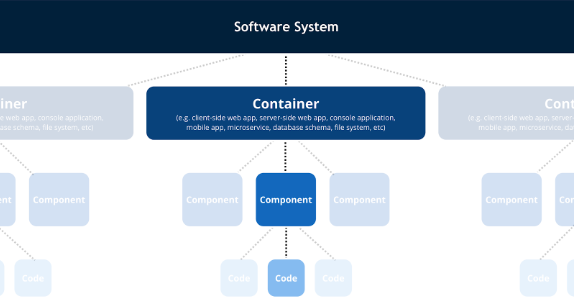
\includegraphics[width=\linewidth]{./img/C4Model.png}
                    \caption[C4 Modell - allgemein]{Das C4 Modell visualisiert ein Komplettsystem durch die Aufgliederung in Teilsysteme.\label{fig:C4}}
                \end{figure}

				\newpage
                \subsubsection*{System Context}
                    Die oberste Position im C4 Modell auf dieses Projekt bezogen wird durch den Anwender belegt, also zum Beispiel einem 
                    Tonmeister. Dieser kann die Audioquellen via Reaper (MultiEncoder) oder HoloLens-Applikation beeinflussen. 
                    Änderungen an einer der beiden Softwaresysteme werden mit 
                    der jeweils anderen synchronisiert (Abb. 
                    \ref{fig:systemContext}).
                    \begin{figure}[htbp]
                        \centering
                        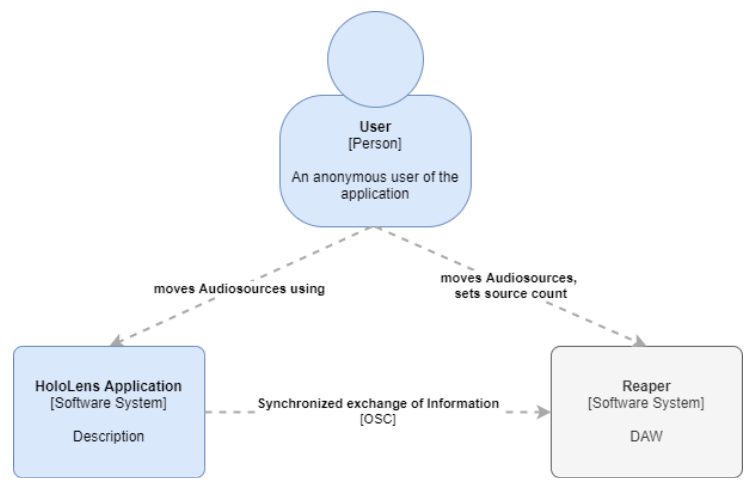
\includegraphics[width=7.5cm]{./img/systemContext.png}
                        \caption[C4 Modell - System Context]{Unabhängig vom Ort der Befehlseingabe synchronisieren sich die Systeme.\label{fig:systemContext}}
                    \end{figure}
                \subsubsection*{Container}
                    Die mit diesem Projekt entwickelte HoloLens-Applikation basiert auf zwei Softwarepaketen. Zum Einen auf dem MRTK für 
                    den Inhalt der Szene in Unity (siehe \ref{sec:2.3.2Video}), 
                    zum Anderen 
                    auf \textit{OSCSimpl} für die Kommunikation im Netzwerk 
                    (siehe \ref{sec:2.3.3Daten}). 
                    Beide Container setzen sich wiederum aus mehreren Komponenten zusammen.
                    \begin{figure}[H]
                        \centering
                        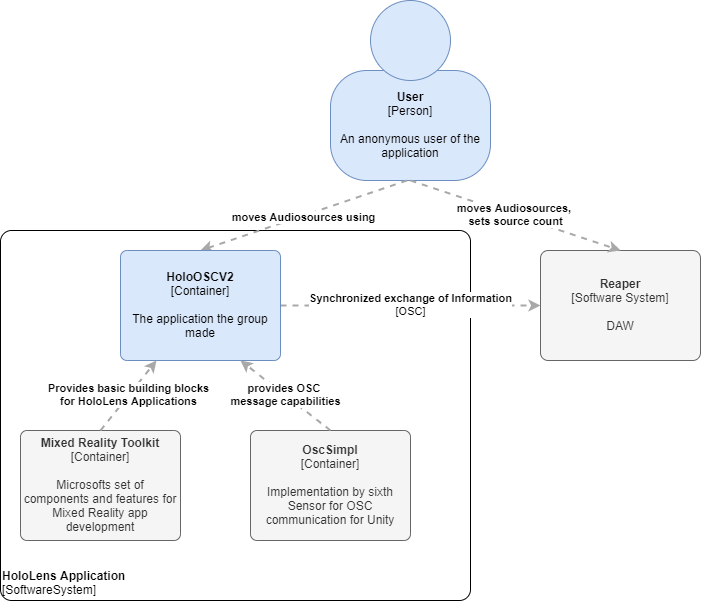
\includegraphics[width=10cm]{./img/C4_Containers.png}
                        \caption[C4 Modell - Container]{Das Zusammenspiel von MRTK und OSCSimpl als Grundlage der Applikation. \label{fig:containerPic}}
                    \end{figure}
                \subsubsection*{Component}
                    Die Szene der AR-Applikation besteht aus mehreren Objekten. Der Anwender selbst befindet sich in einer 
                    Gitternetzkugel (\textit{"'Shell"}). Diese stellt die 
                    Ausdehnung des Lautsprecher-Arrangements dar. Sichtbar sind 
                    weiterhin 
                    die im Multiencoder eingestellten Kanäle in Form von 
                    kleineren Kugeln (\textit{“Sources”}) auf der Hülle der 
                    Gitternetzkugel 
                    sowie eine Benutzeroberfläche mit Schaltflächen und Verbindungsanzeige. In der Szene ebenfalls vorhanden, jedoch 
                    für den Anwender nicht sichtbar sind der 
                    \textit{SourceHandler} und der \textit{OSC Handler}.
                    Dies sind die Komponenten der oben genannten Container. Diese Objekte sind weiterhin ebenfalls mit mehreren Skripten 
                    belegt, deren Funktionen sich in Parameterberechnungen und Nachrichtenverarbeitung spezialisieren. 
                    \begin{figure}[H]
                        \centering
                        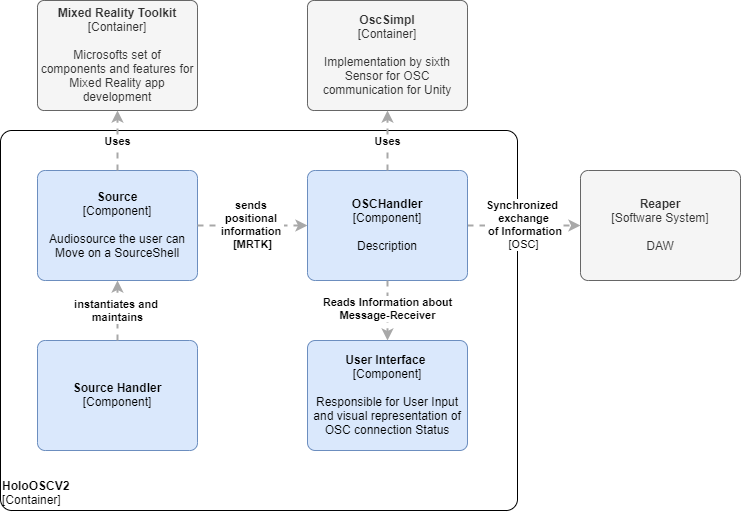
\includegraphics[width=\linewidth]{./img/C4_Components.png}
                        \caption[C4 Modell - Componenten]{Unity-Objekte der AR-Anwendung (blau hinterlegt) als Komponenten übergeordneter Softwarepakete zur Koordination von Informationen.\label{fig:container}}
                    \end{figure}\newpage
            \subsection{OSC-Verbindung zwischen Unity und IEM MultiEncoder}
            \label{sec:3.2.2}
                Wie im letzten Abschnitt beschrieben, sind \textit{SourceHandler} und \textit{OSC Handler} unsichtbare Objekte in der Szene. 
                Für den Verbindungsaufbau ist der \textit{OSC Handler} 
                verantwortlich. Dieser besteht aus fünf Skripten, deren 
                Zusammenwirken 
                außerdem das Empfangen, Verteilen und Versenden von Nachrichten ermöglicht. 
                \subsubsection{Darstellung der Kommunikation via OSC}
                    Die folgenden zwei Abbildungen zeigen schematisch die Verbindungen der einzelnen Elemente. Skripte des \textit{OSC-Handlers} 
                    sind grün hinterlegt und werden anschließend erläutert.
                    \vspace{1cm}
                    \begin{figure}[htbp]
                        \centering
                        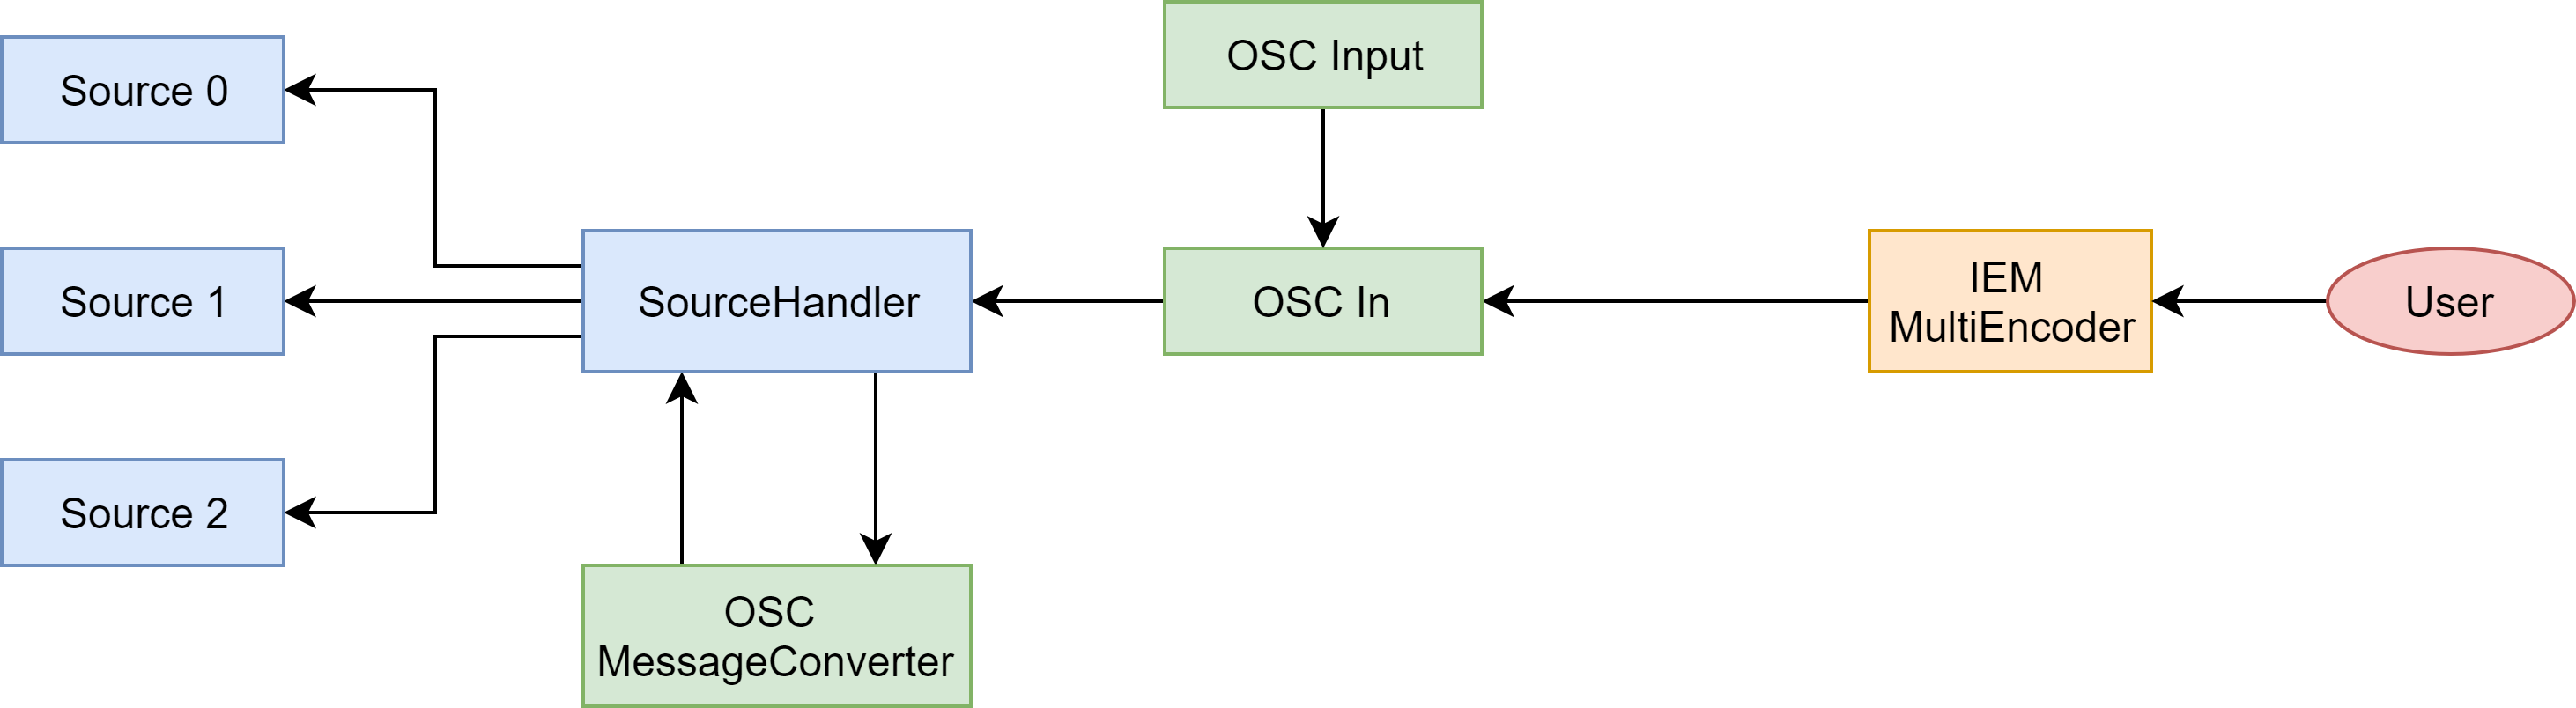
\includegraphics[width=\linewidth]{./img/eingehend.png}
                        \caption{Darstellung der Verarbeitung eingehender OSC-Nachrichten.\label{fig:in}}
                    \end{figure}
                \vspace{1cm}
                    \begin{figure}[htbp]
                        \centering
                        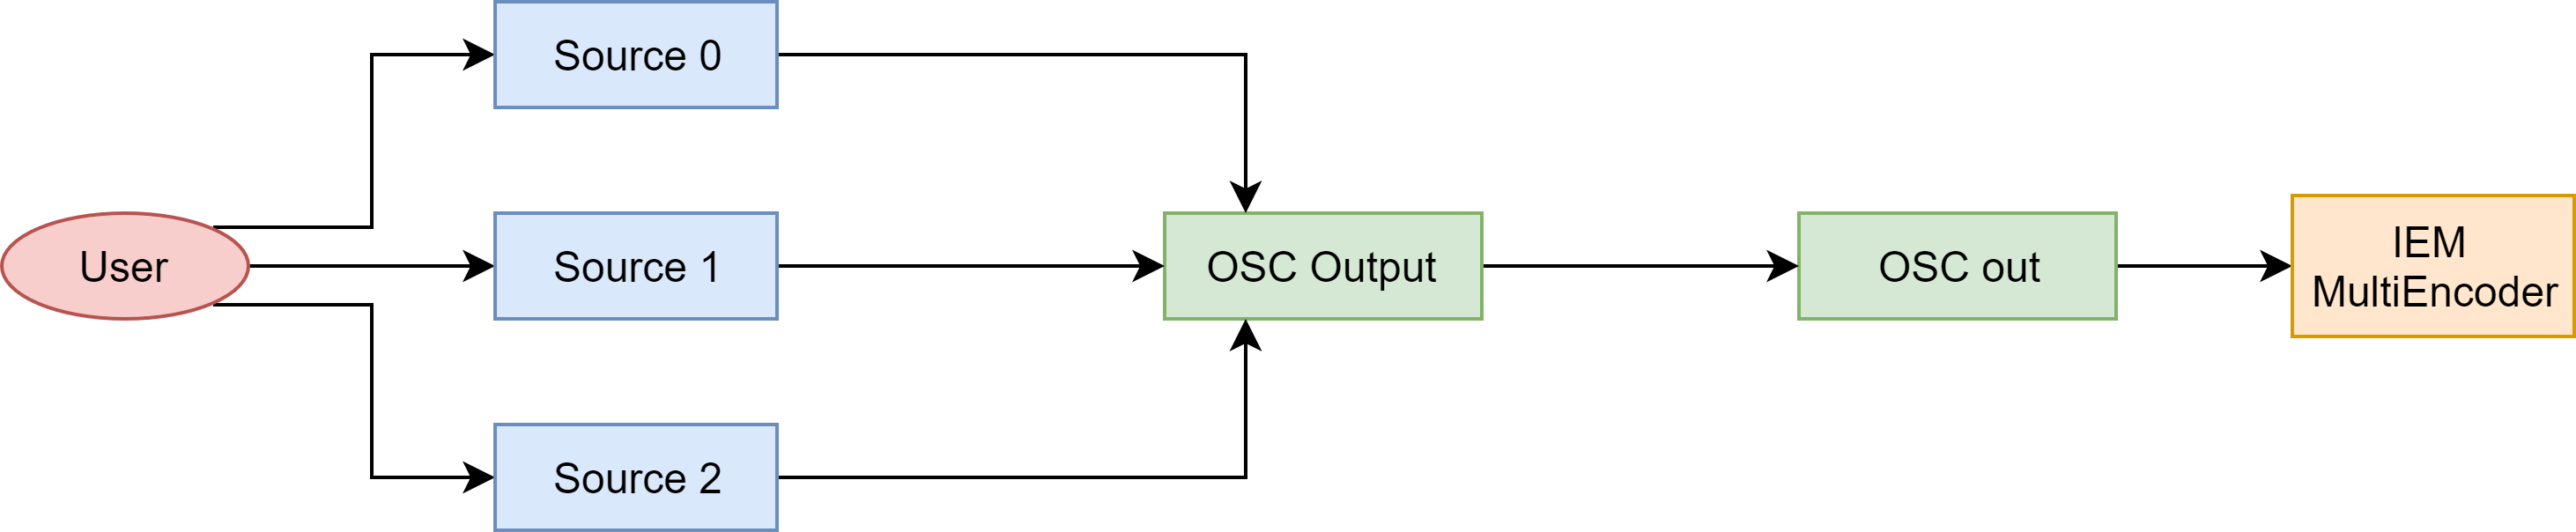
\includegraphics[width=\linewidth]{./img/ausgehend.png}
                        \caption{Darstellung der Verarbeitung ausgehender 
                        OSC-Nachrichten.\label{fig:out}}
                    \end{figure}
                	\pagebreak
                \subsubsection{Bestandteile des OSC-Handlers}
                    \paragraph{Skript - OSC Out}
                    Dieses Skript ist Teil des Assets \textit{OSC Simpl} und 
                    bietet Methoden zum Senden von OSC Nachrichten. 
                    In dieser Anwendung  also die Parameter der einzelnen Kanäle für den MultiEncoder in Reaper. 
                    Gameobjects mit diesem Skript sind OSC Clients. Daher benötigt es die IP Adresse und Port des 
                    Empfängers, in diesem Falle also des Rechners auf dem Reaper läuft. Es können weitere Einstellungen 
                    zur Art und Weise des Sendens vorgenommen werden, die hier nicht weiter genannt werden.
                    Ist der \textit{OSC Handler} in Unity ausgewählt, so werden 
                    im Inspector bei diesem Skript in einem 
                    Nachrichtenfenster alle ausgehenden Nachrichten aufgelistet.
                    \paragraph{Skript - OSC Output} 
                    Um Eingaben der HoloLens für die Netzwerkverbindung korrekt 
                    auszuwerten, wird dieses Skript benötigt. 
                    Es beinhaltet Methoden zur Initiierung von 
                    Verbindungsaufbau und -aktualisierung. Diese werden über 
                    Schaltflächen in der Szene gesteuert. Die in der Anwendung eingegebene IP und Port werden durch den 
                    \textit{ReceiverAdressConverter} umgewandelt, sodass 
                    \textit{OSC Out} benutzt werden kann.
                    \paragraph{Skript - OSC In}     
                    Auch dieses Skript ist Teil von OSC Simpl und bietet 
                    Methoden zum Empfangen von OSC-Nachrichten. 
                    Gameobjects mit diesem Skript sind OSC-Server. Um den 
                    OSC-Server zu starten, muss lediglich ein 
                    Port geöffnet werden. Dieser muss den entsprechenden Angaben im MultiEncoder unter \textit{OSC Sender} 
                    gleichen (siehe Abb. \ref{fig:MultiEncoder}). Eingehende Nachrichten werden mit einer Map in für \textit{Unity nutzbaren} Code 
                    umgewandelt. 
                    Auch hier befindet sich sichtbar auf dem \textit{OSC Handler} ein Nachrichtenfenster in dem alle eingehenden 
                    Informationen gelistet sind.
                    \paragraph{Skript - OSC Input}
                    Dieses Skript öffnet den Port zum Empfangen von Nachrichten und erstellt Maps für \textit{OSC In}. Dadurch werden 
                    Informationen von \textit{OSC In} angepasst und an den \textit{SourceHandler} übergeben.
                    \paragraph{Skript - OSC Message Converter}
                    Damit der \textit{SourceHandler} die eingegangenen 
                    Nachrichten auswerten kann, um die richtigen Werte an die 
                    entsprechende \textit{Source} weiterzuleiten, wird dieses 
                    Skript benötigt. Es zerlegt jede Nachricht in Adresse, 
                    Kanalnummer, Parameter und Wert.
                \subsubsection{OSC im Multiencoder}
                    In der hier verwendeten Version (siehe \ref{sec:secMultiEncoder}) sind im MultiEncoder lediglich die Ports bzw. IP Adressen des 
                    Ein- und Ausgangs festlegbar. Es kann zusätzlich der in der Adresse vorkommende Name vorgegeben werden. 
                    Das Sendeverhalten an sich jedoch, kann nicht beeinflusst werden. Bei Änderung eines Wertes auf einem der 
                    Kanäle wird genau nur diese Änderung als Nachricht verschickt. Auf Knopfdruck “Flush Params” (vergl. Abb \ref{fig:MultiEncoder}) sendet der MultiEncoder 
                    alle Werte von allen Kanälen nacheinander. Bei vierundsechzig Kanälen mit je drei Werten werden entsprechend knapp 
                    zweihundert Nachrichten verschickt, auch wenn nur ein Kanal aktiv ist. Eine direkte Abfrage von Werten ist nach 
                    aktuellem Stand nicht möglich.
                    \pagebreak
                \subsubsection{Connection Status}
                    Die Verbindungsanzeige befindet sich äußerst rechts im User Interface und signalisiert dem Benutzer den aktuellen Verbindungsstatus. 
                    Da es bisher keine Möglichkeit gibt ohne Änderung eines 
                    Wertes Informationen vom MultiEncoder zu bekommen, besteht 
                    die Verbindungsabfrage aktuell aus der Benutzung des 
                    letzten Kanals. Regelmäßig wechselndes Stummschalten des 
                    Kanals dient hier als provisorischer Ping.
                    \begin{figure}[htbp]
                        \centering
                        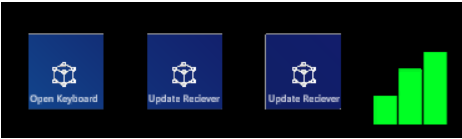
\includegraphics[width=6cm]{./img/status.png}
                        \caption[Die Verbindungsanzeige in der Benutzeroberfläche]{ Aktueller Screenshot der Benutzeroberfläche, äußerst rechts die Verbindungsanzeige.
                        \label{fig:status}}
                    \end{figure} 
            \subsection{Berechnung und Auswertung der Parameter}
            \label{sec:3.2.3}
                Die Szene, in der sich der Nutzer mit der HoloLens bewegt 
                besteht aus einer \textit{SourceShell}, die das Gestell der 
                Lautsprecherarrangierung im 3D-Audio-Labor darstellt (hier eine 
                Gitterneztkugel), sowie aus kleineren Kugeln, die die 
                Schallquellen bzw. Kanäle des MultiEncoders darstellen. Diese Kugeln bewegen sich ausschließlich auf der Hülle der 
                \textit{SourceShell} deren Zentrum durch die Position im Raum 
                der HoloLens beim Laden der Szene festgelegt wird. Gleiches 
                gilt für die Ausrichtung des globalen Koordinatensystems der Szene.
                \subsubsection{Bestimmung und Festlegung von Azimuth und Elevation}
                    Durch den \textit{SourceHandler} eingehende Werte für Elevation und Azimuth sind aufgrund der Nachricht vom 
                    MultiEncoder in Winkel angegeben. Der Radius der Hülle, die 
                    den Dimensionen der Lautsprecheranordnung angepasst ist, 
                    ist im Code 
                    bereits definiert. Durch zwei Winkel und einem Radius lässt sich die Position im Raum genau beschreiben. 
                    Die betroffene Source wandelt diese mit Hilfe des \textit{CoordinateTransformService} in Kartesische 
                    Koordinaten um und definiert somit ihre Position in der 
                    Szene. Ändert sich jedoch die Position einer Quelle in der 
                    Szene durch den Nutzer der HoloLens, werden ihre aktuellen 
                    kartesischen Koordinaten in Kugelkoordinaten umgerechnet und an \textit{OSC Output} gesendet.
                    \begin{wrapfigure}{l}{0.45\textwidth}
                        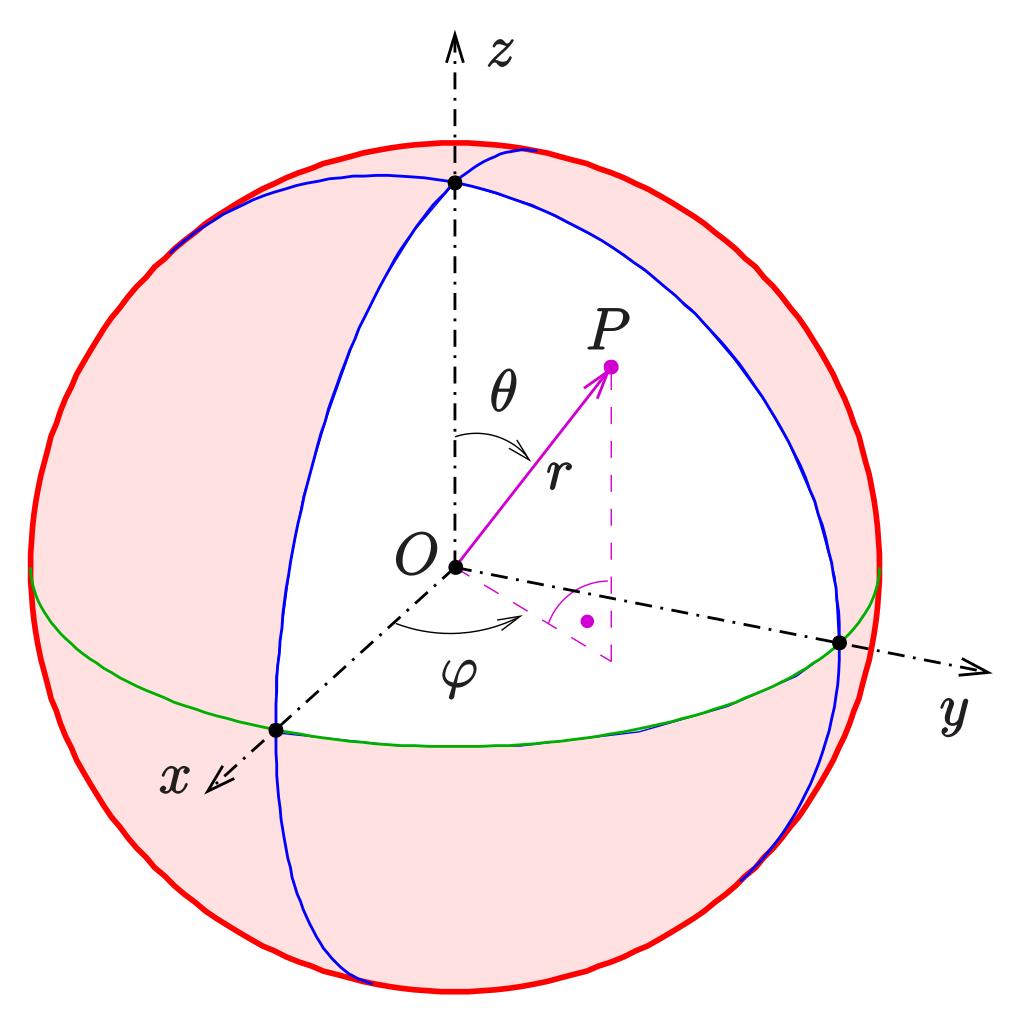
\includegraphics[height=5.5cm]{./img/kugel.png}
                        \caption[Allgemeine Darstellung kartesischer und sphärischer Koordinaten.]
                        {Allgemeine Darstellung kartesischer und sphärischer 
                        Koordinaten.\label{fig:kugel}}
                    \end{wrapfigure}\linebreak
                    \fussy Hier gilt es zu beachten, dass die Koordinaten in \textit{Unity} anders als auf dem Bild dargestellt, 
                    ausgerichtet sind. Die Abbildung repräsentiert daher nicht 
                    die folgenden im Code verwendeten Formeln! 
                    [Wikipedia:Kugelkoordinaten\cite{Kugel}]
                    In \textit{Unity} ist die Y-Achse vertikal und die horizontale Ebene wird durch die X- und Z-Achse aufgespannt.
                    Der MultiEncoder rechnet mit der Elevation, abgebildet ist jedoch die Inklination.\newline\newline
                    \large 
                    $Px=r*\cos(\Theta)*\sin(-\varphi)$ \newline
                    $Py=r*\sin(\Theta)$ \newline
                    $Pz=r*\cos(\Theta)*\cos(-\varphi)$ \newline\newline
                    $\Theta = \arcsin(\frac{y}{r})$\newline
                    $\varphi =-\atantwo(x,z)$\normalsize\newline
                \subsubsection{Grafische Darstellung des Lautstärkepegels (Gain)}
                    Die Werte des Gains im MultiEncoder befinden sich zwischen minus sechzig und plus zehn Dezibel. Damit die Szene 
                    übersichtlich und wortwörtlich greifbar für den Anwender bleibt, wird die Dynamik der Größenveränderung stark eingeschränkt. 
                    Auf jeder \textit{Source} in der Szene befindet sich das 
                    Skript \textit{TransformScaleHandler}. Dieses ist 
                    Bestandteil des 
                    MRTK und dient der Festlegung eines Minimal- und Maximalwertes zur Skalierung einer Kugel. 
                    Die Umrechnung der Werte übernimmt die \textit{Source} selbst. Eingehende Werte werden in den positiven Zahlenbereich verschoben, 
                    auf den vorgegebenen Dynamikumfang der Szene normiert und auf den Minimalwert addiert. Ausgehende Werte werden dementsprechend 
                    wieder auf den höheren Dynamikumfang des MultiEncoders skaliert und um sechzig Werte in den negativen Zahlenbereich verschoben. 
                    Durch diese Umrechnung entstehen aufgrund des Verhaltens von Fließkommazahlen minimale Abweichungen, die jedoch gering und 
                    somit nicht weiter zu betrachten sind.\newline
                    Kugeln im Raum, die auf den Minimalwert skaliert sind, haben im MultiEncoder den Wert -60 dB und sind somit stumm. 
                    Daher wechselt ihre Farbe in der Szene um es ebenfalls übersichtlicher für den Anwender zu machen.
            \subsection{Tooltips zur Kanalzuordnung}
            \label{sec:3.3.4}
                Damit der Benutzer innerhalb der Szene erkennen kann, welche 
                Kugel zu welchem Kanal gehört, wurden Tooltips implementiert. 
                Das \textit{Tooltip-GameObject} ist ein Child des \textit{Source}-GameObject-Prefabs um die Positionen im Raum 
                von Kugel und Tooltip zu verbinden. Da sich alle \textit{Sources} im \textit{SourceHandler} in 
                einem Array befinden und die \textit{Source-ID} gemäß ihrer Position im Array vergeben wird, 
                sind \textit{Source-ID} und Tooltiptext um eins verschoben. (Source-ID “0” als erste Kugel hat also den Tooltip “1” für Kanal “1”).   
            \subsection{Entwicklungsszene in Unity}
            \label{sec:3.2.5}
                Um dem Benutzer ein Zurücksetzen der Szene zu ermöglichen wurde 
                eine Schaltfläche implementiert, welche die Kugeln auf ihre 
                Ursprungspositionen zurückgesetzt und diese ebenfalls an Reaper 
                übermittelt. Dies wurde über eine separate Methode im 
                \textit{ResetScene} Skript realisiert. Damit ein Ändern der IP 
                und des Ports auch in der Szene 
                möglich ist, wurden für diesen Zweck zwei Textfelder implementiert. Durch einen Klick auf den \textit{UpdateReciever} Button wird der 
                Inhalt der Textfelder als neue IP und Port an das \textit{OSCHandler} GameObject 
                gesendet und somit durch das \textit{OSC Out} Skript als neue Empfangsadresse aktualisiert.
    \chapter{Zusammenfassung}% Kapitel 4
    \label{sec:org12d8e10}
    In diesem Kapitel werden zunächst kurz die Ergebnisse zusammengefasst. 
    Darauf folgt die Diskussion, in der Probleme dieser Arbeit angesprochen 
    werden. Abschließend wird ein Ausblick gegeben, wie in dem Projekt 
    weitergearbeitet werden könnte.
        \section{Ergebnis}
        \label{sec:4.1}
        	\sloppy\nohyphens{Vor Beginn des Projekts lag eine erste Version 
        	des Programms vor. 
        	In dieser Version war es bereits möglich, Nachrichten von Unity an 
        	Reaper zu senden. Die Berechnungen von Azimuth und Elevation waren 
        	allerdings nicht korrekt. Weiterhin war es nicht möglich, die 
        	Anzahl der Kanäle zwischen den beiden Programmen zu 
        	synchronisieren.
        	Die Ziele dieser Arbeit bestanden also darin, die bekannten Fehler 
        	zu beheben, sowie neue Features hinzuzufügen. Die geplanten neuen 
        	Funktionen bestanden aus der Möglichkeit, Nachrichten vom 
        	MultiEncoder zu Empfangen und im Programm auszuwerten. Dazu sollte 
        	der Parameter Gain in die Anwendung implementiert werden.\newline 
        	Weiterhin 
        	bestand der Plan, die Intuitivität der Anwendung zu verbessern und 
        	den Entwicklungsprozesses durch Einführung einer Entwickler-Szene 
        	zu optimieren.
        	Durch Koordinatentransformation wurde die fehlerhafte 
        	Positionsberechnung behoben.
        	Zur bereits vorhandenen Funktion, Nachrichten aus der Anwendung an 
        	Reaper zu senden, wurde das Empfangen von Nachrichten ebenfalls 
        	implementiert.\newline Darüber hinaus werden nun die ankommenden 
        	Nachrichten ausgewertet, in die wichtigen Bestandteile zerlegt und 
        	diese dann in einer für die Quellen nutzbare Form 
        	weitergeleitet.
        	Die Abfragen der Kanalanzahl sowie die Parameter der einzelnen 
        	Kanäle aus dem MultiEncoder sind nun möglich.
        	Durch Einsatz beider Hände lässt sich nun der Pegel der einzelnen 
        	Quellen in der HoloLens manipulieren. Diese Skalierung wurde in 
        	Grenzen gesetzt, damit das Projekt in der HoloLens übersichtlich 
        	bleibt. Der Pegelwert wird durch Größe und Farbe der Kugel 
        	dargestellt.\newline
        	Um die Übersichtlichkeit zu verbessern, wurden Tooltips 
        	hinzugefügt, die jeder Kugel ihre Kanalnummer im MultiEncoder 
        	zuweisen. Auch wurde eine Anzeige zum Verbindungsstatus 
        	hinzugefügt.
        	Die Entwicklungsumgebung in Form einer Entwicklerszene ist 
        	vorhanden, konnte aus zeitlichen Gründen allerdings nicht getestet 
        	werden und bietet somit nur einen Grundbaustein für spätere 
        	Weiterarbeit.}\newpage
        \section{Diskussion}
        \label{sec:4.2}
        	Die Bedienung der HoloLens ist nur durch viel Übung 
        	annehmbar.
        	In dieser Applikation ist es notwendig, manuell eine Verbindung zu 
        	einem Empfänger der OSC-Nachrichten aufzubauen. Dazu muss der 
        	Benutzer einen Button drücken, durch den die Systemtastatur der 
        	HoloLens aufgerufen wird. 
        	Der Nutzer muss nun den Zielpunkt der HoloLens auf die Taste 
        	bewegen, die gedrückt werden soll - Finger werden in der HoloLens 
        	noch nicht erkannt, was ein gewöhnliches Zehn-Finger-Schreiben 
        	unmöglich macht.
        	Dazu kommt, dass die Systemtastatur der HoloLens fehlerhaft ist. 
        	Sollte die Tastatur mehr als einmal zur Laufzeit aufgerufen werden, 
        	verschieben sich einige Tasten, diese sind dann auch nicht mehr zu 
        	nutzen. Dies wurde bereits im Juli 2019 auf der offiziellen 
        	Github-Seite des MRTK festgehalten. [Issue @ MRTK Github 
        	\cite{MRTKGit}] 
        	\begin{figure}[H]
        		\centering
        		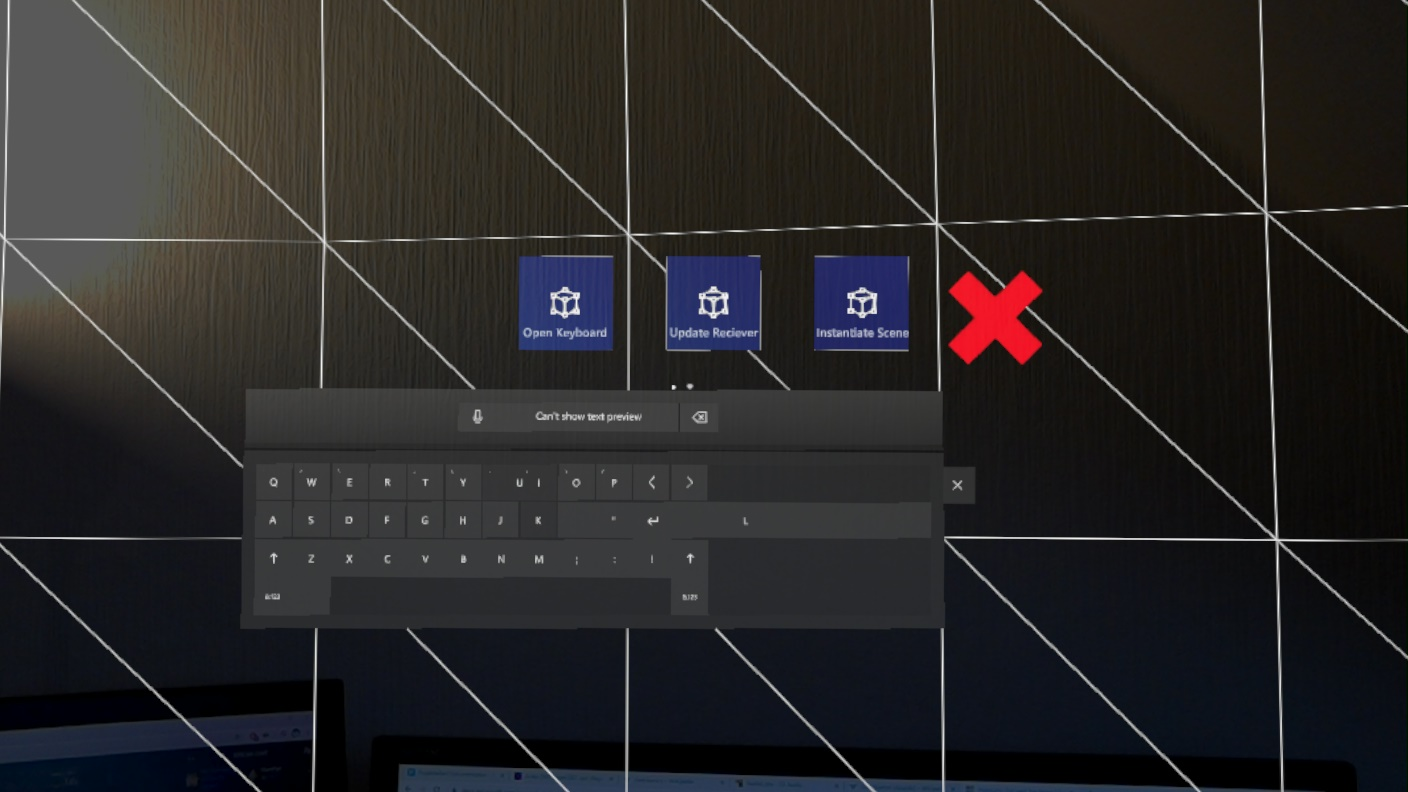
\includegraphics[width=0.8\linewidth]{./img/KeyBoardBug.jpg}
        		\caption{Darstellung eines Bugs der internen Tastatur der 
        			HoloLens \label{fig:Keyboard}}
        	\end{figure}
        	%[https://github.com/microsoft/MixedRealityToolkit-Unity/issues/5169]
        	Ebenso ist es uns im Projekt weder gelungen, eine Voransicht des 
        	getippten für den Nutzer sichtbar zu machen, noch eine Korrektur 
        	des getippten zu ermöglichen. Sollte sich der Teilnehmer 
        	vertippen, muss die Tastatur neu aufgerufen werden, um die Eingabe 
        	neu vorzunehmen. \newline
        	Des Weiteren ist die Implementierung der Spracheingabe nicht 
        	praktikabel. Im Hauptmenü der HoloLens lassen sich die meisten 
        	Applikationen auch per Sprache steuern, was in der Anwendung zu 
        	Problemen geführt hat. Der Nutzer hatte für kurze Zeit die 
        	Möglichkeit, statt den Button zur Aktualisierung des Empfängers zu 
        	drücken, diesen auch per Sprachkommando “Update Receiver” zu 
        	nutzen. Diese Funktion musste wieder entfernt werden, da die 
        	Anwendung bei mehreren eigenen Sprachkommandos durcheinander kam. 
        	So wurde kurzzeitig das Sprachkommando “Open Keyboard” ebenfalls 
        	implementiert, die Anwendung vertauschte diese Kommandos aber oft, 
        	was wiederum zu einer negativen User Experience führt.\newline
        	Ein wichtiger Aspekt der Softwareentwicklung, der in diesem Projekt 
        	fast vollständig vernachlässigt worden ist, ist das Unit-testing. 
        	Gewöhnlicherweise ist das Testen der Applikation fester Bestandteil 
        	des Softwareentwicklungsprozesses. Neben Unit-tests werden auch 
        	Integrations-Tests und System-Integrationstests parallel zur 
        	Entwicklung neuen Codes durchgeführt. Jegliches Testen in diesem 
        	Projekt erfolgte jedoch ausschließlich über Klicktests. Jede 
        	Änderung wurde manuell vom Entwickler selbst getestet.\newline Die 
        	Projektgruppe versuchte zumindest das Unit-testing in den 
        	Entwicklungsprozess unterzubringen, allerdings konnte das 
        	Testing-Framework NUnit nicht erfolgreich genutzt werden.
        	Beim Versuch über die IDE Unit-Tests zu starten kam es zu der 
        	Fehlermeldung “ ‘feature out of variable declaration’ is not 
        	available in C\#6”. Nach gründlicher Prüfung der Fehlermeldung ist 
        	es uns nicht gelungen, diesen Fehler zu beheben, was zur Folge hat, 
        	dass wir keine Unit-Tests ausführen konnten.\newline
        	Durch dieses Projekt sollte eine möglichst identische Abbildung des 
        	IEM-MultiEncoders in der HoloLens dargestellt werden. Zu einer 
        	möglichst einfachen Bedienung bedarf es einer synchronen 
        	Darstellung der Werte in der Applikation und im MultiEncoder. 
        	Allerdings sendet das MultiEncoder-Plug-in nicht automatisch 
        	Nachrichten via OSC, sondern nur nach einer Änderung.
        	Durch diese Eigenschaft der OSC-Verbindung seitens des 
        	MultiEncoders ist das Laden einer bestehenden Szene äußerst 
        	schwierig. 
        	Der Nutzer startet die Applikation in der HoloLens und öffnet 
        	Reaper. In Reaper wird ein Audioprojekt geladen. Der Nutzer stellt 
        	eine OSC-Verbindung zwischen der HoloLens und Reaper her. Daraufhin 
        	ändert sich in der Applikation auf der HoloLens nichts - da in 
        	Reaper keine Änderungen vorgenommen worden sind, werden auch keine 
        	Werte übertragen.\newline
        	Die verwendete OSC-Implementation OscSimpl ist noch in der 
        	Entwicklungsphase. Erst im Verlauf der Arbeit wurde es möglich, 
        	über die HoloLens OSC-Nachrichten zu empfangen. Dies war bis dahin 
        	nicht möglich, da OscSimpl das Mappen von Daten mit 
        	Unity-Funktionen implementierte, die veraltet waren. Die veralteten 
        	Unity-Funktionen sind für Unity selbst unproblematisch, die 
        	Anwendung kann OSC-Nachrichten über die Entwicklungsumgebung 
        	unproblematisch senden und empfangen. Allerdings ist dies auf der 
        	HoloLens nicht möglich, ein Update war zwingend notwendig. Das 
        	neueste Update ist allerdings nicht nur auf die veralteten 
        	Mapping-Funktionen beschränkt - Es werden nun alle OSC-Nachrichten 
        	als Bundle verschickt und empfangen. Dadurch entstand ein neues 
        	Problem: Gesendete Nachrichten, die kurz hintereinander verschickt 
        	werden, gehen auf dem Übertragungsweg verloren. Im Unity-Forum 
        	[OSC simpl Forum, Beitrag \#87 \cite{OscSimpl87}] wurde auf diesen 
        	Fehler aufmerksam gemacht und 
        	dieser ist angeblich seit Ende Dezember 2019 gelöst. Dies ist jedoch 
        	nicht der Fall, OSC-Nachrichten gehen weiterhin auf dem Sendeweg 
        	verloren. Bis zum Ende des Projekts ist es uns nicht gelungen, 
        	beide Übertragungsrichtungen für OSC auf der HoloLens verfügbar zu 
        	machen.
        	
        \section{Ausblick}
        \label{sec:4.3}
        	Am Ende der Arbeit stehen noch einige Verbesserungen in Sachen 
        	Benutzerfreundlichkeit offen. Zum Einen mangelt es an 
        	Fehlermeldungen, zur Problembeschreibung. Diese sollten zusammen 
        	mit der Behebung oben genannter Probleme Aufgaben einer 
        	Weiterarbeit an diesem Projekt sein. Zum Anderen gilt es die 
        	Entwicklerszene zu erweitern oder überarbeiten, damit das 
        	Testen neuer Features erleichtert und somit beschleunigt 
        	wird.\newline
        	Durch die HoloLens2 werden die Interaktionen innerhalb der 
        	AR-Umgebung deutlich angenehmer für den Nutzer. Durch das Wegfallen 
        	des Zielpunktes und der verbesserten Fingererkennung ist zum 
        	Beispiel die Bedienung einer Tastatur wesentlich einfacher. Dadurch 
        	ergeben sich neue Möglichkeiten andere Plug-ins anzusteuern, die 
        	eine feinere Bedienung benötigen.\newline
        	Da der Datenverkehr über OSC simpl stattfindet und dieser Weg 
        	Probleme mit der HoloLens aufzeigt, ergeben sich 2 Möglichkeiten, 
        	dieses Problem in Zukunft anzugehen. Entweder es wird auf einen 
        	Patch gewartet (siehe OSC simpl Forum \cite{OscSimpl87}) oder 
        	zukünftige Arbeitsgruppen finden eine Alternative zu OSC 
        	simple.\newline
        	Derzeit wird in der Anwendung nur eine Spur mit bis zu 64 Kanälen 
        	angesteuert. In der Realität werden oft mehrere Spuren in einem 
        	Projekt verwendet. Daher gilt es herauszufinden, wie mehrere 
        	Plug-ins zeitgleich angesteuert werden können.\newline
        	Damit die Fehlersuche und -analyse in der HoloLens selbst 
        	vereinfacht 
        	wird, ist es sinnvoll eine Debugeinheit in das Interface zu 
        	implementieren. Somit kann die Anwendung auch auf der HoloLens 
        	produktiv getestet werden. Weiterhin können so Fehler aufgedeckt 
        	werden, die nur während der Bedienung des Gerätes, nicht aber beim 
        	Testen in der Entwicklungsumgebung auftauchen.\newline
        	Neben den bisher implementierten Parametern können zusätzlich die 
        	Optionen für das Stumm- oder Soloschalten der einzelnen Kanäle 
        	hinzugefügt werden. Dies könnte beispielsweise mit einem 
        	Kontextmenü beim Klick auf die Kugeln 
        	realisiert werden.\newpage
            
  \printbibliography       

\end{document}